\documentclass[12pt,a4paper]{article}
\usepackage{graphicx}
\usepackage[margin=1.2in]{geometry}
\usepackage{amsmath}
\usepackage{array}
\usepackage{multirow}
\usepackage{textcomp}
\usepackage{graphicx}



\begin{document}
\title{\textbf {PHYS 9702}}
\date{Waves}
\maketitle
\tableofcontents{}
\section*{Notes}
\textit{This study guide was prepared by Dyandra Charismiadji based on lectures by Frans A. Rambe in 2018 - 2019 along with additional information from the Second Edition AS/A-Level Physics Coursebook and workbook, various websites, and youtube. It is provided as-is and may contain errors, though effort has been made to minimize this. }

\newpage
\section{Waves}
\subsection{Longtitudinal waves}
\begin{itemize}
    \item Particles of medium vibrate \textit{parallel} to the direction of wave velocity.
    \item Examples: sound waves.
    \item These waves require a medium to travel (e.g. sound waves require air).
\end{itemize}
\subsection{Transversal waves}
\begin{itemize}
    \item Particles of medium vibrate at \textit{right angles} (\textbf{90}\textdegree) to the direction of wave velocity.
    \item Examples: light waves and electromagnetic waves.
    \item Due to the direction of its particles movement, these waves can be \textit{polarized}.
\end{itemize}
\subsection{Calculations involving waves}

\subsubsection{The Doppler effect}
An effect that occurs when the source and/or sink of the wave is in motion.

\begin{center}
\begin{tabular}{ |c|c| } 
 \hline
 \textbf{Observer in Motion} & \textbf{Source in Motion}  \\ 
\hline
 $f_o = \frac{V \pm V_o}{V}f_s$ & $f_o = \frac{V}{V \pm V_s}f_s$  \\ 
\hline
 \textbf{$+ V_o$} = toward source & \textbf{$+ V_s$} = away sink  \\ 
 \textbf{$- V_o$} = away source & \textbf{$- V_s$} = toward sink  \\
 \hline
\end{tabular}
\end{center}

\begin{center}
\begin{tabular}{ | l | l | } 
 \hline
 \multicolumn{2}{|c|}{\textbf{Observer and Source in Motion}}\\
 \hline
\hline
\multirow{4}{7em}{$f_o = f_s(\frac{V \pm V_o}{V \pm V_s})$} & \textbf{$+ V_o$} = toward source \\ 
& \textbf{$- V_o$} = away source \\
& \textbf{$+ V_s$} = away sink \\ 
& \textbf{$- V_s$} = toward sink \\ 
\hline
\end{tabular}
\end{center}

\noindent V = speed of sound in air (330 m/s)

\subsection{Electromagnetic waves}

\begin{figure}[h]
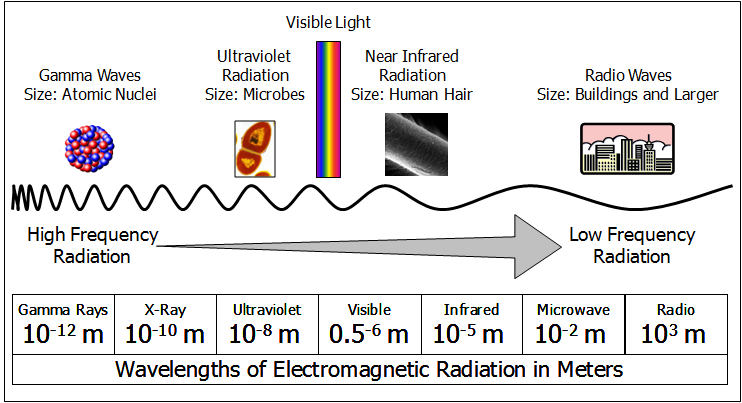
\includegraphics[width=0.75\textwidth]{graphics/em_spectrum.png}
\centering
\end{figure}

\newpage
\section{Superposition of Waves}
\noindent
\textbf{Superposition} occurs when two or more waves overlap, resulting in the \textit{algebraic sum} of the individual waves.

\bigskip \noindent
\textbf{Phase Difference} is the fractional part of a period which represents the offset in peak positions of waves.
%% insert sample question here

\bigskip \noindent
\textbf{Coherence} between phases of two or more waves causes \textit{stationary interference} to be able to be observed. TL/DR: Coherence causes two waves to become \textit{stationary} (i.e. they have a constant phase difference and the same frequency, and the same waveform).
\subsection{Diffraction}
\textbf{Diffraction} is the spreading of a wave as it passes through a gap. 

\smallskip \noindent 
\textbf{Diffraction Effects} are greater when waves pass through a gap with a width \textit{roughly equal to their wavelength}. Examples:
\begin{itemize}
    \item \textbf{Soundwaves} can spread through doorways because the width of a doorway is comparable to the wavelength of a soundwave. 
    \item Due to their small wavelength, \textbf{visible light}'s diffraction can be observed by passing it through a \textit{very small slit}.
    \item \textbf{Radio waves} can have wavelengths of the order of a kilometer, so they can easily be diffracted by gaps in hills, tall buildings, etc.
    \item Cars need \textbf{external radio aerials} because radio waves are too big to be diffracted by car windows.
    \item A \textbf{microwave oven} uses a metal grid with tiny gaps behind its glass display to allow us to see the food inside but keep the microwaves (with $\lambda$ of 12.5 cm) in.
\end{itemize}

\begin{figure}[h]
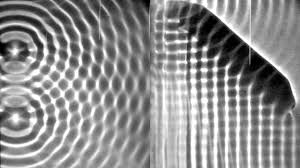
\includegraphics[width=7cm]{graphics/ripplenipple.jpg}
\centering
\end{figure}

To explain diffraction simply, think of water ripples. In some directions, the ripples \textit{add together}; in others, they \textit{cancel out}.

\subsection{Interference}
\textbf{Interference} is the variation with distance or time of the amplitude due to superposition of two or more waves.
\begin{itemize}
    \item \textbf{Constructive}: resultant amplitude \textbf{greater than} either individual wave.
    \item \textbf{Destructive}: resultant amplitude \textbf{lesser than} either individual wave.
\end{itemize}  
\begin{center}
\begin{tabular}{ | l | l | } 
 \hline
 \multicolumn{2}{|c|}{\textbf{Path Difference}}\\
 \hline
\hline
 \textbf{Constructive Interference} & \textbf{Destructive Waves}\\ 
\hline
 $0$, $\lambda$, $2\lambda$, $3\lambda$, etc. & $\frac{1}{2}\lambda$, $1\frac{1}{2}\lambda$, $2\frac{1}{2}\lambda$, etc.\\ 
\hline
 $n\lambda$ & $(n + \frac{1}{2})\lambda$\\
\hline
\end{tabular}
\end{center}

\begin{figure}[h]
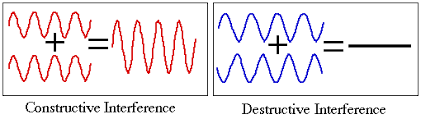
\includegraphics[width=10cm]{graphics/destructive_constructive.png}
\centering
\caption{Destructive and constructive interference.}
\end{figure}

\subsubsection{Interference of sound waves}
When two loudspeakers produce waves of a single wavelength, the sound is \textbf{louder} in some points and \textbf{quieter} in others. 

\begin{figure}[h]
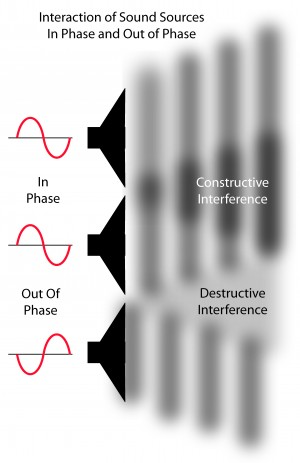
\includegraphics[width=5cm]{graphics/sound_interference.jpg}
\centering
\caption{Interference in sound waves.}
\end{figure}

\bigskip \noindent
\textbf{Loud sound}	$\rightarrow$ $|d_1 - d_2|$ = $n\lambda$

\smallskip \noindent
\textbf{Soft sound}	$\rightarrow$ $|d_1 - d_2|$ = $(\frac{2n + 1}{2})\lambda$
\subsubsection{Interference of microwaves}

\subsection{The Young double-slit experiment}
In order to observe interference, the sources of waves must be \textit{coherent}. We can achieve this by passing a single beam of light through two slits

\bigskip \noindent
\textbf{Diffraction} spreads the light outwards, resulting in two waves even though there is a single source.

\bigskip \noindent
\textbf{Interference} occurs due to the waves overlapping. This results in the interference fringes observed. The presence of bright spots are caused by constructive interference, while the dark spots are caused by destructive interference.

\subsection{Diffraction gratings}

\begin{figure}[h]
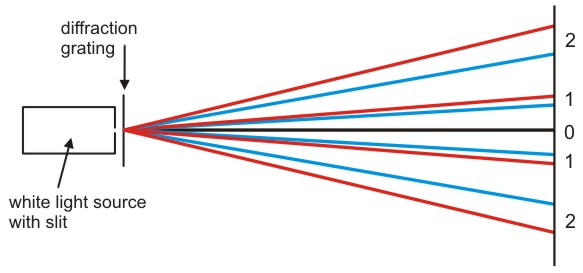
\includegraphics[width=0.5\textwidth]{graphics/diffraction_grating.jpg}
\centering
\end{figure}

\begin{center}
Use $\frac{ax}{D} = n\lambda$ or $asin\theta = n\lambda$
\end{center}

\newpage
\section{Stationary Waves}
\textbf{Stationary Waves} are the result of the superposition of two progressive waves. The two progressive waves must have: 
\begin{itemize}
    \item equal \textbf{amplitude}
    \item equal \textbf{frequency}
    \item same \textbf{speed}
    \item \textbf{opposite direction}
\end{itemize}
The two waves must also be completely \textbf{out of phase} (phase difference = \textbf{180}\textdegree)

\subsection{Nodes and antinodes}
\textbf{Nodes} are points along the wave that do not move.

\smallskip\noindent
\textbf{Antinodes} are points along the wave that move with maximum displacement.

\begin{figure}[h]
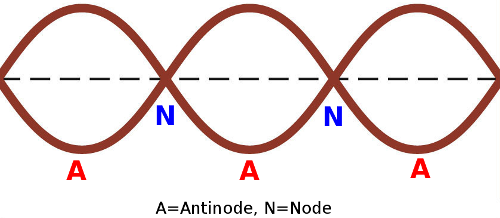
\includegraphics[width=7cm]{graphics/node_antinode.png}
\centering
\end{figure}

\subsection{Calculations involving stationary waves}
\subsubsection{Stationary waves and musical instruments}
The wavelength and frequency are affected by the shape of the instrument, i.e. closed tube or open tube.

\begin{figure}[h]
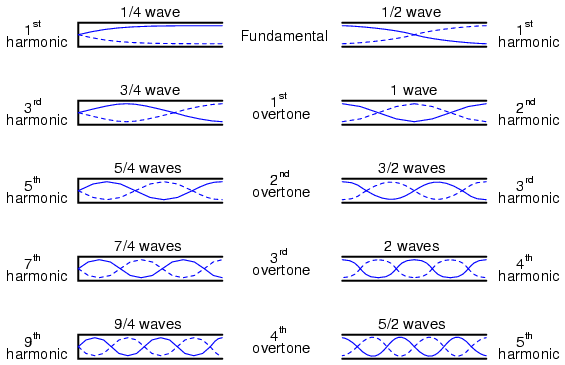
\includegraphics[width=0.5\textwidth]{graphics/tubes.png}
\centering
\end{figure}




\end{document}